\documentclass[10pt, conference, a4paper, final]{IEEEtran}
\IEEEoverridecommandlockouts
\usepackage{amsmath, amssymb}
\usepackage[margin=1in]{geometry} % Adjust margins if needed
\usepackage{graphicx} % Required for including images
\usepackage{subcaption}
\usepackage{algorithm, algorithmicx} % For algorithms
\usepackage[table,xcdraw]{xcolor} % For colored tables
\usepackage{enumitem} % For better control over list
\usepackage{microtype} % Improves typography
\usepackage{amsmath}

% Combine graphicx package loading
\usepackage{float}
\usepackage{booktabs} % For professional looking tables

\title{A Comprehensive Testing Framework for Deep Learning Models}
\author{Author Name}
\date{\today}

\begin{document}

\maketitle

\begin{abstract}
% Your abstract goes here.
\end{abstract}


\section{Introduction}

\section{Problem Statement}

Deep learning models are being more widely used in a variety of applications, yet their reliability in practical applications remains a challenge.


\section{Research Goal}
This paper aims to develop a systematic framework for evaluating local and global robustness in deep learning models. 
The goal is to provide a comprehensive error summary to improve model design and training, ensuring their reliability for real-world applications.

\section{Contributions}
This research makes the following key contributions to the field of deep learning robustness evaluation:
\begin{itemize}
   
    \item We design an \textbf{end-to-end pipeline} for evaluating the robustness of system.
    
    \item We propose a \textbf{conceptual framework} that quantifies both local and global robustness,with formalized approach to verify system robustness.
    \item A novel \textbf{error summarization}  approach which allows better identification of model weaknesses related to class and property.

    \item We perform all our \textbf{experiments} using publicly available deep learning models and MNIST dataset.
\end{itemize}

\section{Research Questions}

This paper addresses the following research questions applicable to various deep learning models and datasets:

\begin{itemize}
    \item How can we design a comprehensive framework to test system robustness?
    \item How can we systematically evaluated the robustness both at local (property-specific) and global (overall system) levels within framework?
    \item How can error summarization be employed to quantify the impacts on model robustness?
 
\end{itemize}


\section{Methodology}
\begin{figure*}{}
    \centering
    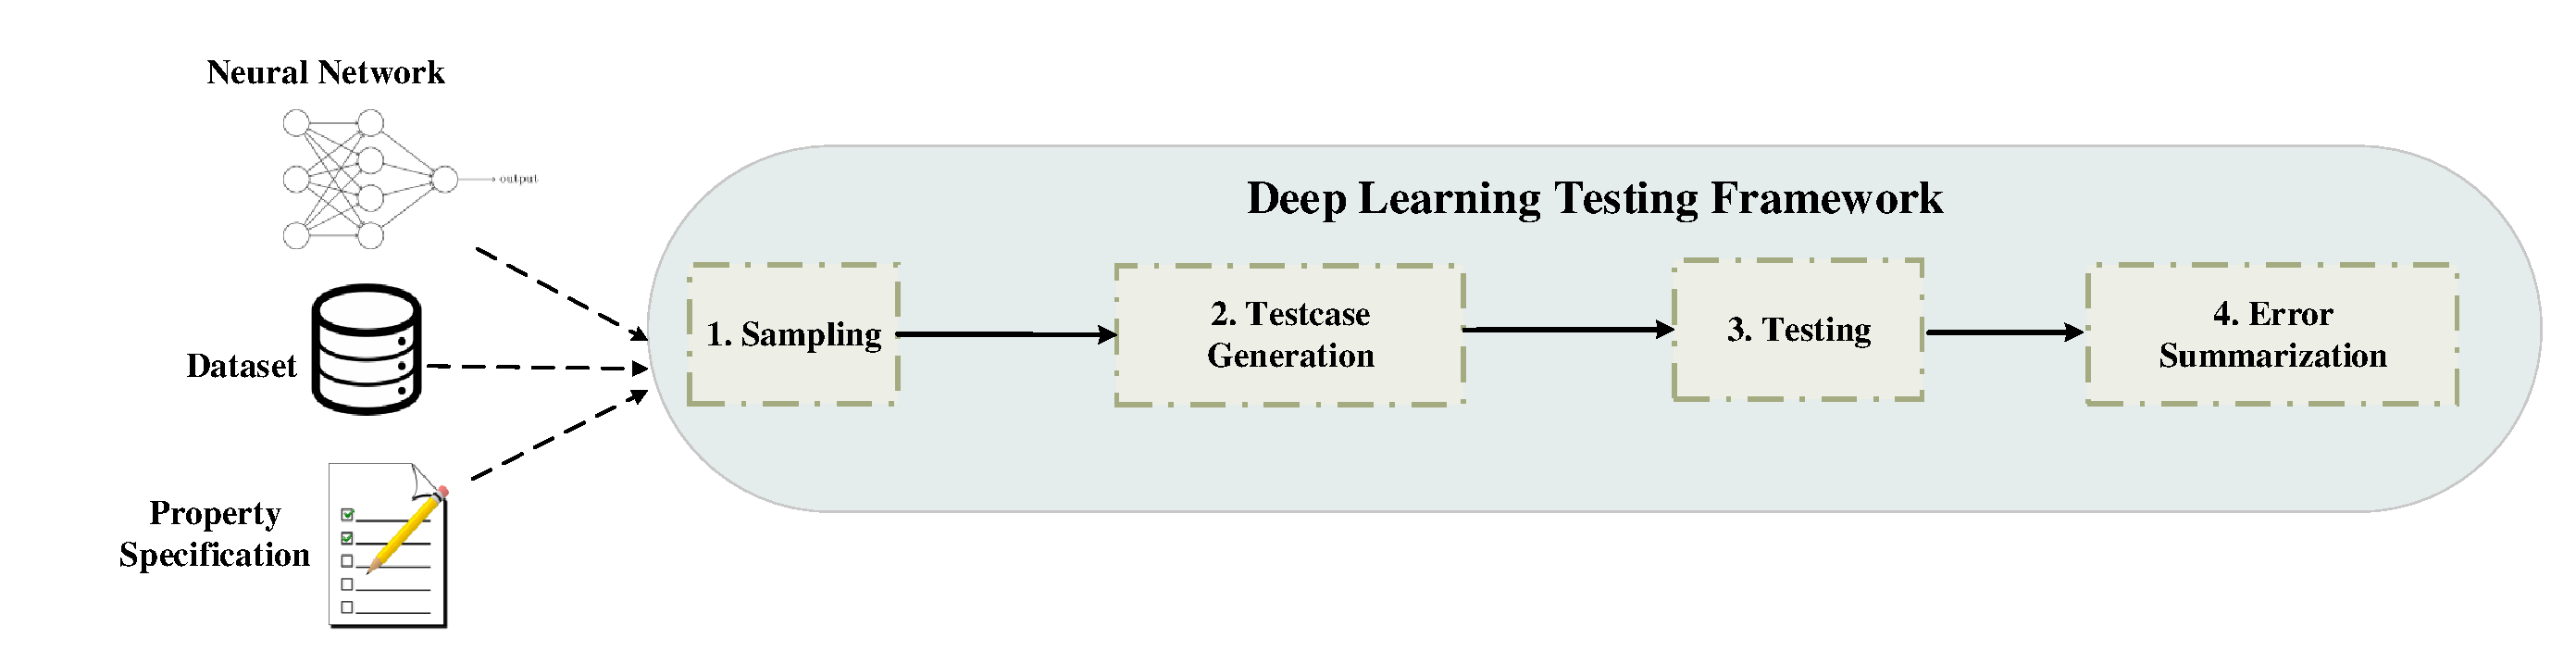
\includegraphics[width=\linewidth]{paper_images/DL framework.pdf}
    \caption{Overview of Testing Framework}
    \label{fig:graph}
\end{figure*}


This section presents an overview of the comprehensive testing framework, which is intended to test the specified properties according to given specification. The pipeline begins by precisely describing the properties to be evaluated. To comprehensively examine the model, test cases are created and tested. The error summary step next concentrating on the progression from local to global robustness to highlight the system systemic strengths and weaknesses. This systematic technique improves the robustness of deep learning models by tackling each essential aspect sequentially, from specification to complete error analysis.

\subsection{Sampling}
 The sample selection process involves a random but balanced choice of samples from each class, focusing exclusively on instances that the model has correctly predicted. This method ensures a representative and fair distribution of data across all classes.

\begin{itemize}

    
        \item Model Utilization:
            \begin{itemize}
                \item A pre-trained CNN model is utilized to select samples.
                \item Let \( X = \{x_1, x_2, \dots, x_N\} \) denote the set of MNIST images. The model function \( f \) predicts:
                \[ f(x_i) \rightarrow y_i \]
                \item The filter function \( g \) identifies accurate predictions, defined as:
                \[ g(x_i) = 
                \begin{cases} 
                1 & \text{if } f(x_i) = \text{true label of } x_i \\
                0 & \text{otherwise}
                \end{cases} \]
                \item The subset \( S \) includes only correctly predicted images:
                \[ S = \{x_i \in X \mid g(x_i) = 1\} \]
            \end{itemize}
        \item Random Selection of Samples:
            \begin{itemize}
                \item Randomly selects 200 samples from each class in \( S \), totaling 2000 samples.
                \item The random selection function \( R \) is defined to ensure:
                \[ R(S_c, 200) \text{ for each class } c \text{ in } S \]
                where \( S_c \) represents the samples of class \( c \) within \( S \).
            \end{itemize}

\end{itemize}


\subsection{Test Case Generation}

This section outlines the generation of test cases to assess model robustness through properties such as noise, rotation, and brightness adjustments.

\begin{figure}{}
    \centering
    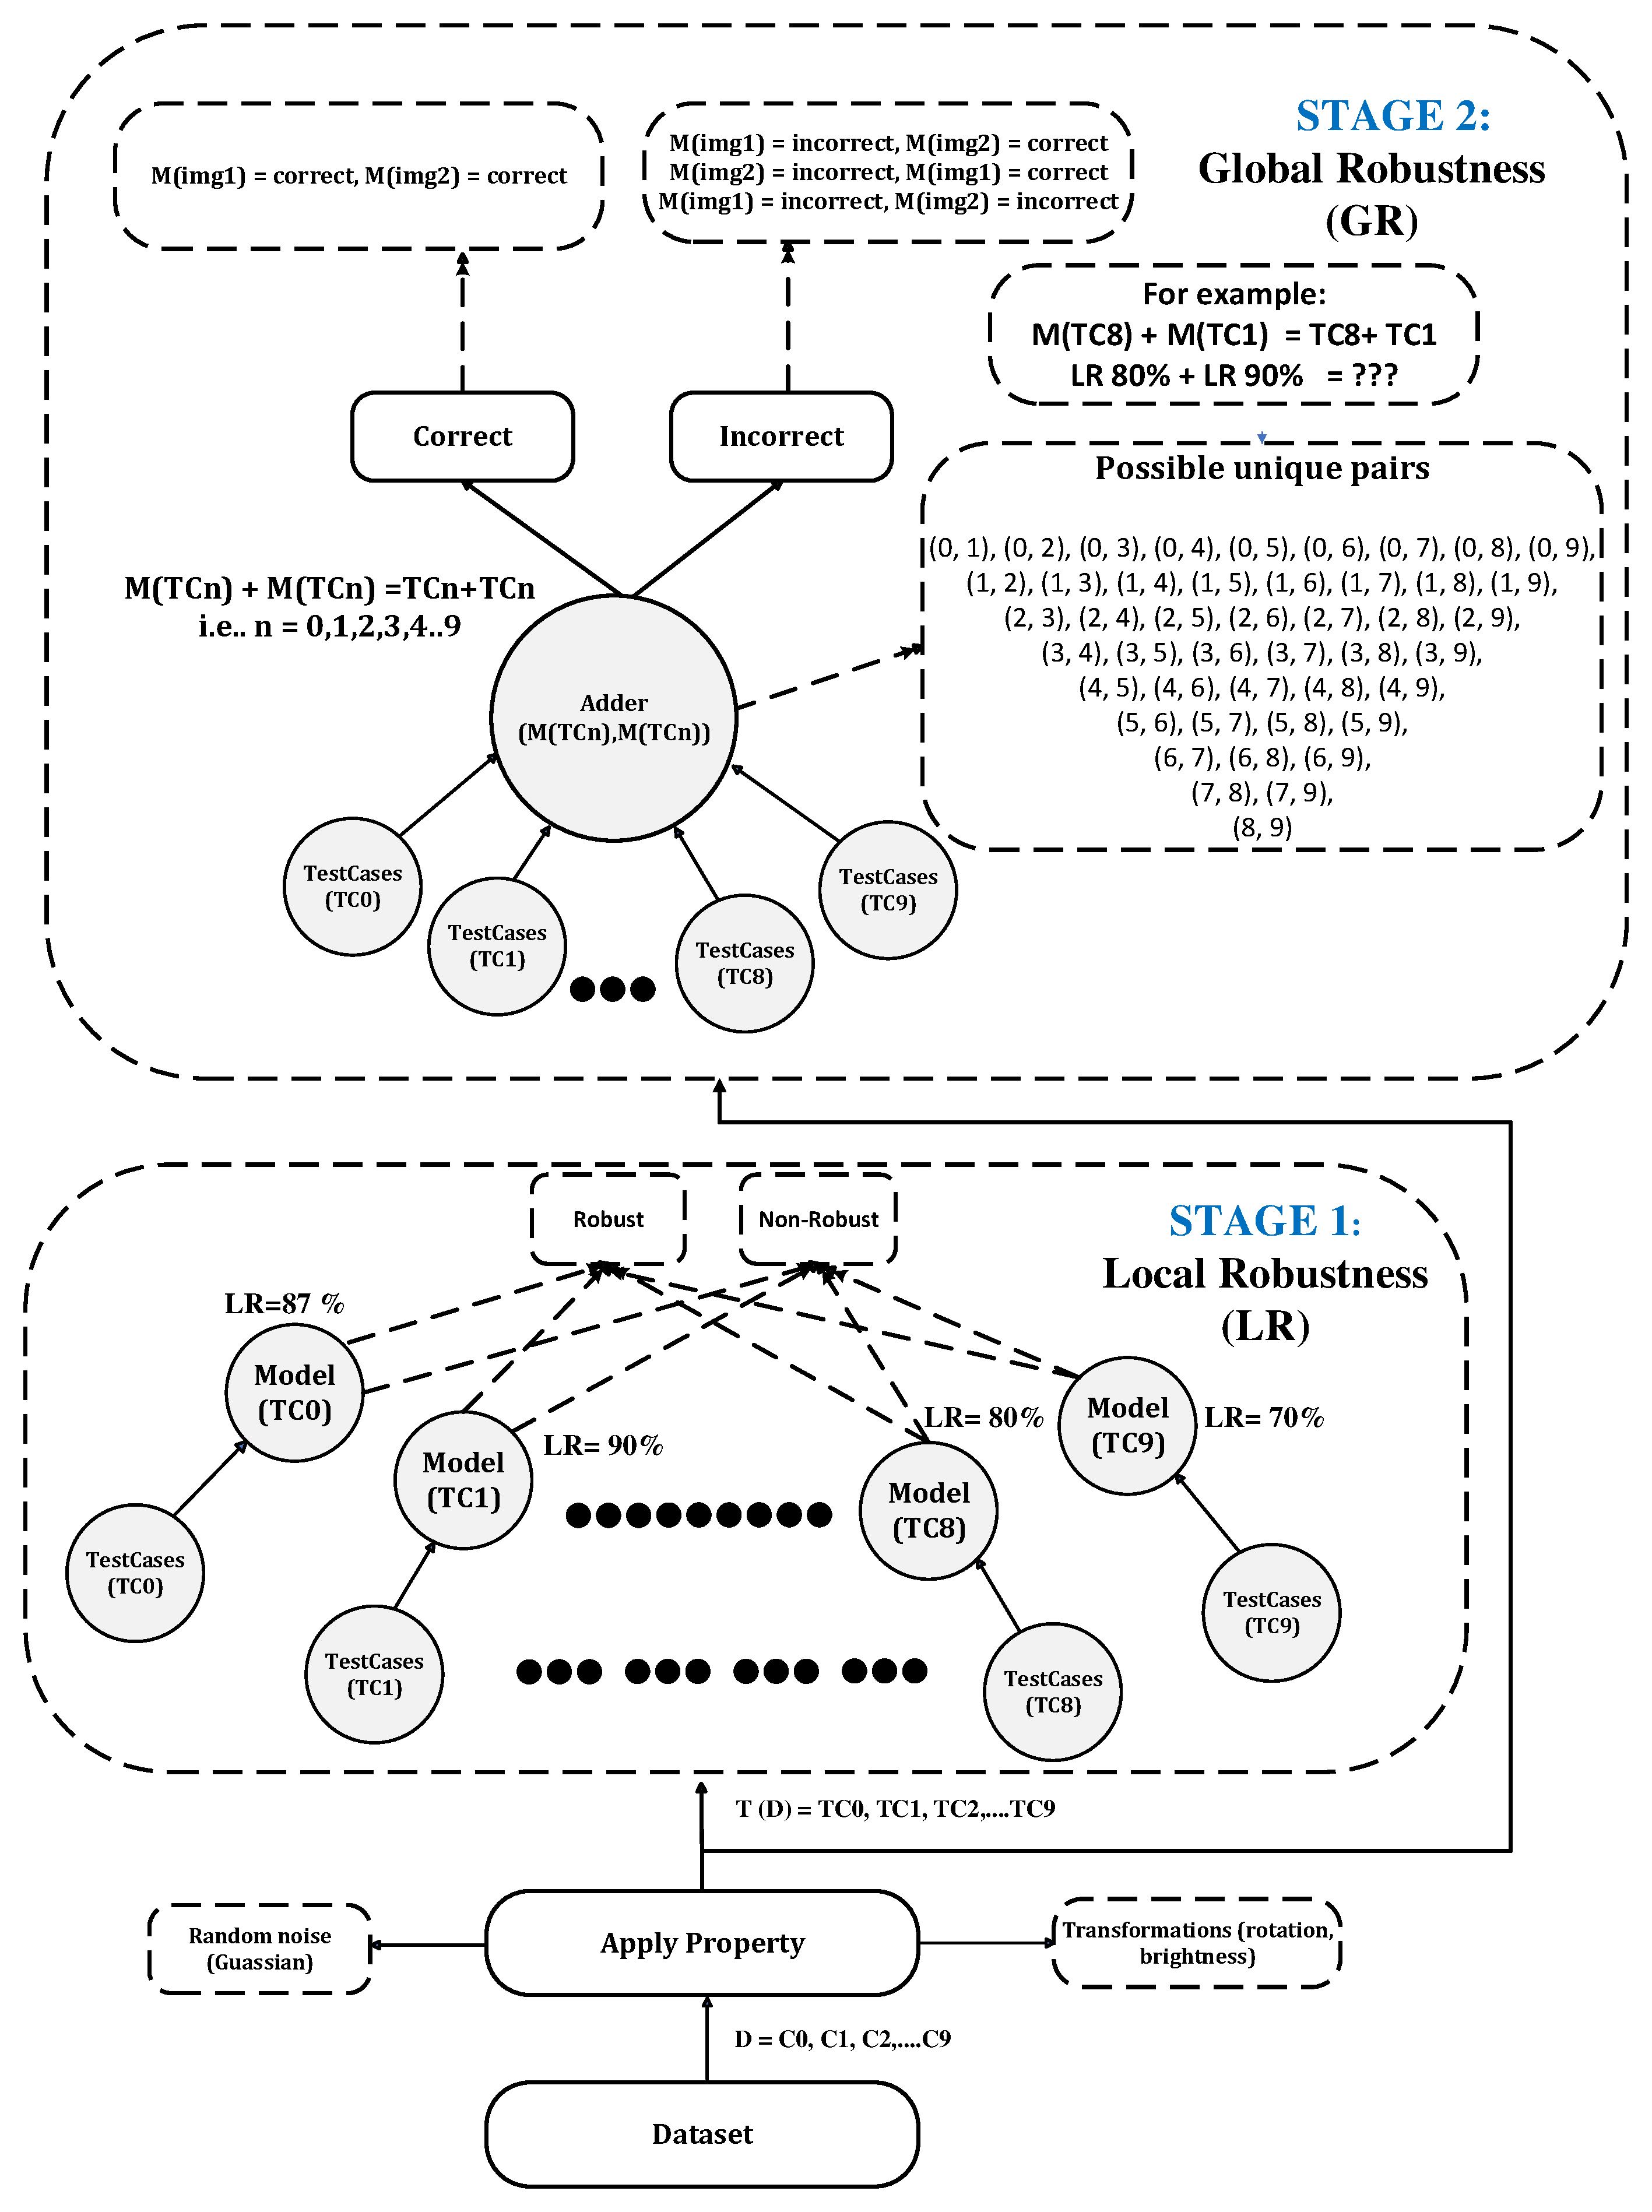
\includegraphics[width=\linewidth]{paper_images/MNIST Adder.pdf}
    \caption{Graphical View of Local and Global Robustness}
    \label{fig:graph}
\end{figure}

\begin{itemize}
    \item \textbf{Noise Addition:} Noise is added to an image \( x_i \) using a Gaussian noise model. The noise function \( p_n \) is defined as:
    \[ p_n(x_i, \sigma) = x_i + \epsilon \]
    where \( \epsilon \sim \mathcal{N}(0, \sigma^2) \) denotes the Gaussian noise with mean zero and standard deviation \(\sigma\).

    \item \textbf{Rotation:} The rotation of an image \( x_i \) by an angle \(\theta\) is modeled by the rotation function \( p_r \):
    \[ p_r(x_i, \theta) = \text{rotate}(x_i, \theta) \]
    where \(\text{rotate}(\cdot, \theta)\) represents the rotation operation.

    \item \textbf{Brightness Adjustment:} Brightness adjustment of an image \( x_i \) is controlled by a multiplicative factor \( \beta \), which scales the intensity of all pixels. The brightness function \( p_b \) can be defined as:
    \[ p_b(x_i, \beta) = \beta \cdot x_i \]
    where \( \beta > 1 \) increases brightness, and \( \beta < 1 \) decreases it. This approach ensures that the image's contrast is preserved while adjusting its brightness.

\end{itemize}

\subsection{Testing }

The Testing section evaluates how accurately and confidently the model predicts under various properties (noise, rotation, brightness) applied to images from each class. This phase focuses on directly measuring and quantifying the robustness of the model.
\begin{itemize}

    \item Confidence Level Assessment:
        \begin{itemize}
            \item After generating test cases, measure the model’s confidence for each class under each type of property.
            \item Aggregate these measurements to assess the overall robustness of individual properties (noise, rotation, brightness).
        \end{itemize}

        \item Local Robustness:
        Local robustness quantifies the robustness of a deep learning model to perturbations in input data, specific to individual properties such as noise, rotation, and brightness. This metric assesses the probability of each class individually when these properties are altered, providing a measure of the model's stability under various conditions.

        \item Definition and Measurement:
        
        Local robustness for a class \(c\) subjected to a property \(p\) is formally defined as the conditional probability of correct classification given the perturbed input:
        \begin{equation}
            LR_{c,p} = P(\hat{Y}_{c,p} = Y_c \mid X_c = x'_{c,p}),
        \end{equation}
        where \(X_c = x'_{c,p}\) represents the application of property \(p\) with parameter \(\theta_p\) to the original image \(x_c\). The property function \(p(x_c, \theta_p)\) modifies the input \(x_c\) accordingly, e.g., adding Gaussian noise or adjusting brightness.

   
        To practically estimate local robustness, the model is tested across a statistically significant number of trials, each involving perturbed inputs. The empirical local robustness is calculated as the average of indicator functions over these trials:
        \begin{equation}
            \hat{LR}_{c,p} = \frac{1}{N} \sum_{i=1}^N \mathbf{1}(f(p(x_{c,i}, \theta_p)) = y_{c,i}),
        \end{equation}
        where \(N\) is the number of test cases, \(f\) denotes the predictive function of the model, and \(\mathbf{1}\) is the indicator function that evaluates to 1 if the condition is true and 0 otherwise.



        \subsection{Global Robustness Evaluation}
        Global robustness assesses the model's ability to correctly process and combine outputs from multiple inputs under identical perturbations, using an "adder function" that sums the predictions. This measure evaluates how well the model integrates and interprets simultaneous input perturbations.
        
        \subsubsection{Definition and Mathematical Formulation}
        
        Global robustness is defined through an adder function that sums the predicted outputs for two inputs subjected to the same perturbation, and compares this sum to the expected combined result:
        \begin{multline}
            GR_{(c1, c2), p} = P(\text{Adder}(\hat{Y}_{c1,p}, \hat{Y}_{c2,p}) = \\
            Y_{\text{combined}} \mid X_{c1} = x'_{c1,p}, X_{c2} = x'_{c2,p})
        \end{multline}
        
        where:
        \begin{itemize}
            \item \(x'_{c1,p}\) and \(x'_{c2,p}\) are the perturbed inputs from classes \(c1\) and \(c2\), respectively, after the application of property \(p\).
            \item \(\hat{Y}_{c1,p}\) and \(\hat{Y}_{c2,p}\) are the predictions for these inputs.
            \item \(\text{Adder}(\hat{Y}_{c1,p}, \hat{Y}_{c2,p})\) represents the function that sums these predictions.
            \item \(Y_{\text{combined}}\) is the expected result of the combined predictions, reflecting correct model output for both inputs together.
        \end{itemize}
        


        \begin{multline}
            \hat{GR} = \frac{1}{M} \sum_{j=1}^M \mathbf{1}(\text{Adder}(f(x'_{j1,p}), f(x'_{j2,p})) \\= Y_{j,\text{combined}})
        \end{multline}
        where:
        \begin{itemize}
            \item \(M\) is the number of test pairs.
            \item \(\mathbf{1}\) is the indicator function that returns 1 if the adder's output matches the combined expected result and 0 otherwise.
            \item \(f\) is the prediction function, and \(x'_{j1,p}\), \(x'_{j2,p}\) are the perturbed images in the \(j\)-th test case.
        \end{itemize}

        
    \end{itemize}

\subsection{Error Summarization}
This section details the error summarization process following the global robustness testing, where we identify and analyze discrepancies in the model's predictions. By tracing errors from the combined outputs back to individual properties and classes, we systematically pinpoint and address underlying weaknesses.

\subsubsection{Example Setup}
We consider two classes from the MNIST dataset:
\begin{itemize}
    \item Class A: Digit `5'
    \item Class B: Digit `0'
\end{itemize}
Both classes are tested under the properties of noise and rotation, with the following local robustness confidence levels:
\begin{itemize}
    \item \( LR_{A,p_1} = 85\% \) (Noise)
    \item \( LR_{A,p_2} = 78\% \) (Rotation)
    \item \( LR_{B,p_1} = 90\% \) (Noise)
    \item \( LR_{B,p_2} = 88\% \) (Rotation)
\end{itemize}

\subsubsection{Global Robustness Testing Scenario}
The model is tasked with processing two images, one from each class, both subjected to noise. The ideal prediction should reflect the sum `5' (Class A) + `0' (Class B) = `5'. An incorrect sum indicates a prediction error.

\subsubsection{Error Summarization Process}

\begin{figure}[H]
    \centering
    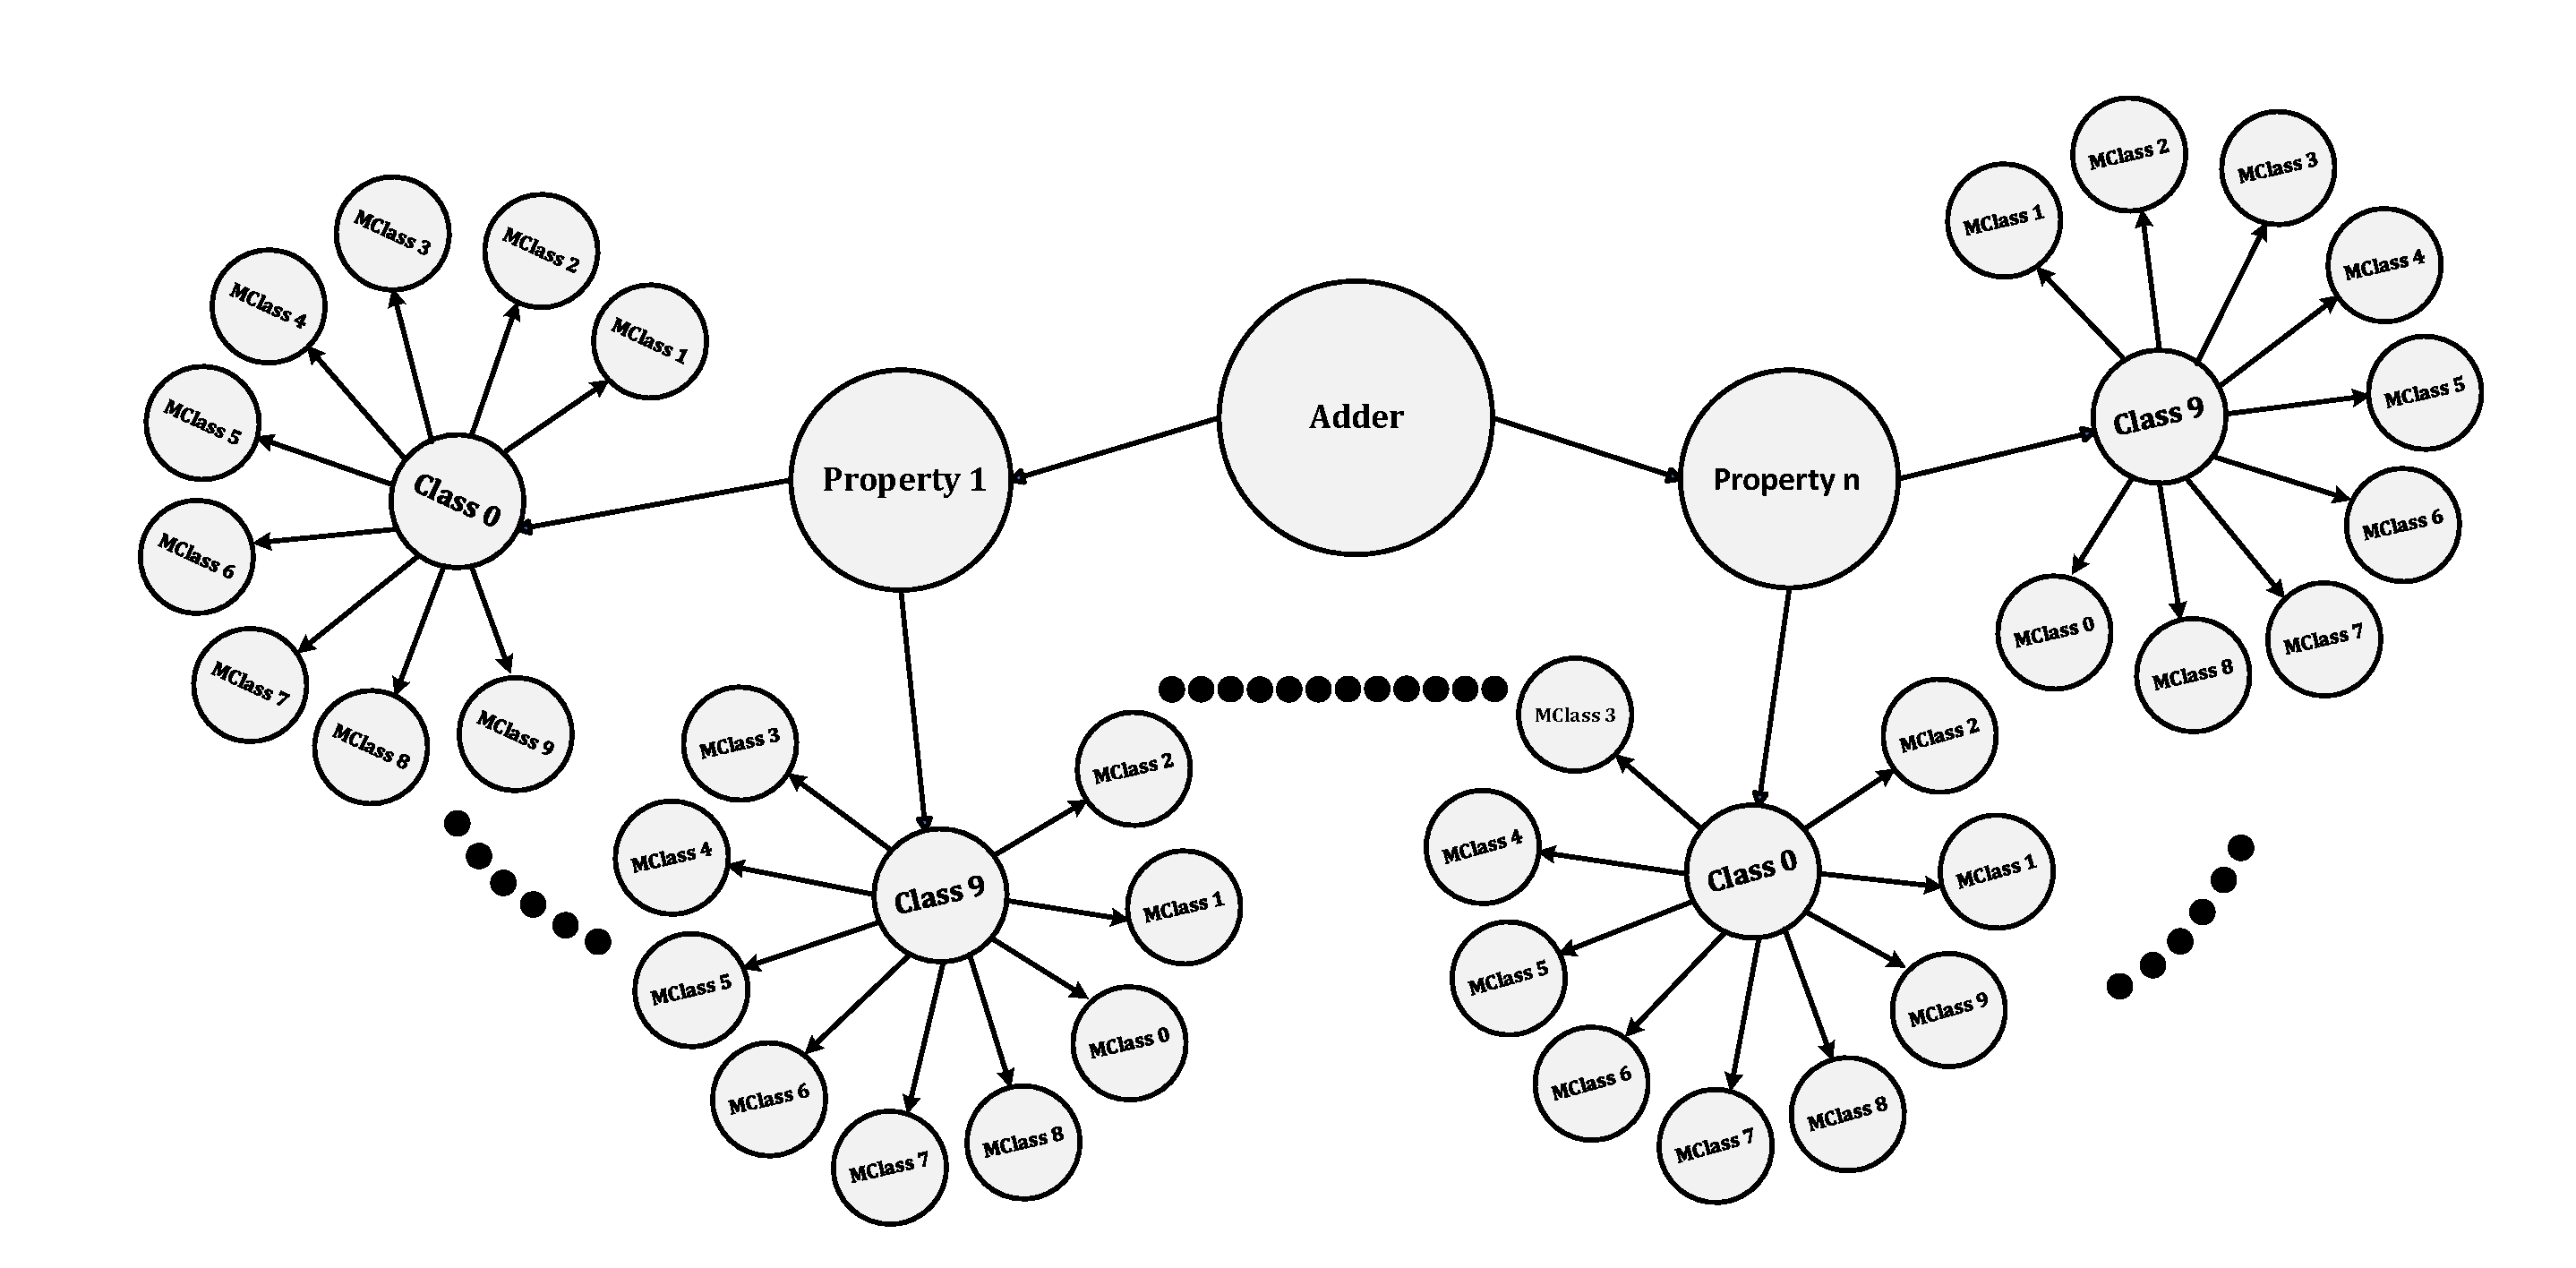
\includegraphics[width=\linewidth]{paper_images/step4.pdf}
    \caption{Diagram of Error Summarization Highlighting Class-Property Impact}
    \label{fig:error-summarization}
\end{figure}



\begin{enumerate}
    \item \textbf{Initial Error Detection:}
        The combined prediction incorrectly sums to `6' instead of `5'.

    \item \textbf{Identify the Inaccurate Predictions:}
        Examination reveals the model predicts `6' for Class A and correctly predicts `0' for Class B.

    \item \textbf{Drill Down to Property Level:}
        Both images were tested under noise. The noise robustness for each class is assessed:
        \begin{itemize}
            \item \( LR_{A,p_1} = 85\% \) — suggesting a 15\% failure rate.
            \item \( LR_{B,p_1} = 90\% \)
        \end{itemize}

    \item \textbf{Assess Individual Local Robustness:}
        Focus is placed on Class A's noise robustness, identifying potential misclassification trends under noisy conditions.

    \item \textbf{Further Analysis:}
        Investigate if certain noise patterns consistently mislead the model concerning digit `5', potentially confusing it with a similar appearance to `6'.

    \item \textbf{Systematic Error Identification:}
        Patterns of error involving Class A under noise are sought to determine if specific adjustments in model training or data handling can mitigate these issues.

    \item \textbf{Propose Adjustments:}
        Modifications to the training process or data augmentation strategies are suggested to enhance noise robustness, especially for digits with appearances similar to `5'.
\end{enumerate}





\section{Experiments}


\section{Threats to Validity}

This section outlines significant limitations and assumptions in our study that may affect the validity and reliability of our findings.

\begin{itemize}
    \item \textbf{Random Sampling:} Our current approach assumes a uniform distribution of samples across all classes, which may not represent the true complexity and variability within real-world data. This uniform sampling can lead to biased evaluations if the class distribution in practical applications is skewed or non-uniform. We plan to enhance our sampling techniques to better capture the diversity and distribution of data in realistic scenarios. Improved sampling strategies will help in developing more robust and generalizable error summarization methods.
\end{itemize}


\section{Related Work}
% Your content here

\section{Conclusion}
% Your conclusion here

\begin{thebibliography}{01}
    \bibitem{Saad} Reference details
\end{thebibliography}

\end{document}
